
\section{shells}

\subsection{shells, the concept}

\begin{frame}{shell}
\begin{itemize}
    \item allow user (= person at keyboard) to run applications
    \item user's wrapper around process-management functions
\end{itemize}
\end{frame}

\begin{frame}{aside: shell forms}
\begin{itemize}
    \item POSIX: command line you have used before
        \vspace{.5cm}
    \item also: graphical shells
        \begin{itemize}
        \item e.g. OS X Finder, Windows explorer
        \end{itemize}
    \item other types of command lines?
    \item completely different interfaces?
\end{itemize}
\end{frame}

\begin{frame}<1>[fragile,label=commandLineFeatures]{some POSIX command-line features}
\begin{itemize}
\item \myemph<2>{searching for programs}
    \begin{itemize}
    \item \verb|ls -l| $\approx$ \verb|/bin/ls -l|
    \item \verb|make| $\approx$ \verb|/usr/bin/make|
    \end{itemize}
\item running in background
    \begin{itemize}
    \item \verb|./someprogram &|
    \end{itemize}
\item \myemph<4>{redirection}:
    \begin{itemize}
    \item \verb|./someprogram >output.txt|
    \item \verb|./someprogram <input.txt|
    \end{itemize}
\item \myemph<5>{pipelines}:
    \begin{itemize}
    \item \verb!./someprogram | ./somefilter!
    \end{itemize}
\end{itemize}
\end{frame}

\againframe<2>{commandLineFeatures}

\begin{frame}[fragile,label=searchForPrograms]{searching for programs}
\begin{itemize}
    \item POSIX convention: PATH \textit{environment variable}
        \begin{itemize}
        \item example: \texttt{/home/cr4bd/bin:/usr/bin:/bin} 
        \item list of directories to check in order
        \end{itemize}
    \item environment variables = key/value pairs stored with process
        \begin{itemize}
        \item by default, left unchanged on execve, fork, etc.
        \end{itemize}
    \item one way to implement:  [pseudocode]
\begin{lstlisting}
for (directory in path) {
    execv(directory + "/" + program_name, argv);
}
\end{lstlisting}
\end{itemize}
\end{frame}


\subsection{I/O redirection: syntax, method preview}

\againframe<4>{commandLineFeatures}

\subsection{pipelines}

\againframe<5>{commandLineFeatures}

\section{files in POSIX, part 1}

\subsection{interlude: file descriptors}

\begin{frame}[fragile,label=fds]{file descriptors}
\begin{lstlisting}[language=C,style=smaller]
struct process_info {
    ...
    struct open_file *files;
};
...
process->files[file_descriptor]
\end{lstlisting}
    \begin{itemize}
    \item Unix: every process has \\
        array (or similar) of \textit{open file descriptions}
    \item ``open file'': \small terminal $\cdot$ socket $\cdot$ regular file $\cdot$ pipe
    \item file descriptor = index into array
        \begin{itemize}
        \item usually what's used with system calls
        \item stdio.h FILE*s usually have file descriptor + buffer
        \end{itemize}
    \end{itemize}
\end{frame}






\begin{frame}{special file descriptors}
\begin{itemize}
\item file descriptor 0 = standard input
\item file descriptor 1 = standard output
\item file descriptor 2 = standard error
\vspace{.5cm}
\item constants in \texttt{unistd.h}
    \begin{itemize} \item \texttt{STDIN\_FILENO}, \texttt{STDOUT\_FILENO}, \texttt{STDERR\_FILENO} \end{itemize}
\vspace{.5cm}
\item<2-> but you can't choose which number \texttt{open} assigns\ldots?
    \begin{itemize}
    \item more on this later
    \end{itemize}
\end{itemize}
\end{frame}



\subsection{getting file descriptors}


\begin{frame}[fragile,label=gettingFds]{getting file descriptors}
\begin{lstlisting}[
    language=C++,
    moredelim={**[is][\btHL<1-|handout:1->]{@1}{1@}},
    style=smaller
]
int read_fd = open("dir/file1", O_RDONLY);
int write_fd = open("/other/file2", O_WRONLY | ...);
int rdwr_fd = open("file3", O_RDWR);
\end{lstlisting}
\begin{itemize}
\item used internally by fopen(), etc.
\item also for files without normal filenames\ldots:
\end{itemize}
\begin{lstlisting}[
    language={},
    moredelim={**[is][\btHL<1-|handout:1->]{@1}{1@}},
    style=smaller,
]
int fd = shm_open("/shared_memory", O_RDWR, 0666); // shared memory
int socket_fd = socket(AF_INET, SOCK_STREAM, 0); // TCP socket
int term_fd = posix_openpt(O_RDWR); // pseudo-terminal
int pipe_fds[2]; pipe(pipefds); // "pipes" (implements ./command | ./other_cmd)
...
\end{lstlisting}
\end{frame}


\subsection{close}

\begin{frame}[fragile,label=close]{close}
\begin{lstlisting}[language=C++]
int close(int fd);
\end{lstlisting}
\begin{itemize}
\item close the file descriptor, deallocating that array index
    \begin{itemize}
    \item does not affect other file descriptors \\ that refer to same ``open file description''
    \item (e.g. in \texttt{fork()}ed child or created via (later) \texttt{dup2})
    \end{itemize}
\item if last file descriptor for open file description, resources deallocated
\vspace{.5cm}
\item returns 0 on success
\item returns -1 on error
    \begin{itemize}
    \item e.g. ran out of disk space while finishing saving file
    \end{itemize}
\end{itemize}
\end{frame}


\subsection{Shell: redirection}

\input{../unix-api/redirection}

\subsection{dup2: redirection mechanism}

\begin{frame}<1>[fragile,label=reassign]{reassigning file descriptors}
\begin{itemize}
\item redirection: \verb|./program >output.txt|
\item step 1: open output.txt for writing, get new file descriptor
\item step 2: \myemph<2>{make that new file descriptor stdout (number 1)}
\vspace{.5cm}
\item<2-> tool: \texttt{int dup2(int oldfd, int newfd)} \\
        make \texttt{newfd} refer to same open file as \texttt{oldfd}
    \begin{itemize}
    \item same \textit{open file description}
    \item shares the current location in the file
    \item (even after more reads/writes)
    \end{itemize}
\item<2-> what if newfd already allocated --- closed, then reused
\end{itemize}
\end{frame}

\begin{frame}[fragile,label=dup2AndTable]{reassigning and file table}
\begin{lstlisting}[language=C,style=smaller]
// something like this in OS code
struct process_info { 
    ...
    struct open_file_description *files[SIZE];
    ....
};
...
process->files[STDOUT_FILENO] = process->files[opened-fd];
\end{lstlisting}
\begin{itemize}
\item syscall: \texttt{dup2(\textit{opened-fd}, STDOUT\_FILENO);}
\end{itemize}
\end{frame}

\againframe<2>{reassign}

\begin{frame}[fragile,label=dup2example]{dup2 example}
redirects stdout to output to \texttt{output.txt}:
\begin{lstlisting}[language=C++,style=small]
fflush(stdout);  /* clear printf's buffer */
int fd = open("output.txt",
              O_WRONLY | O_CREAT | O_TRUNC);
if (fd < 0)
    do_something_about_error();

dup2(fd, STDOUT_FILENO);
/* now both write(fd, ...) and write(STDOUT_FILENO, ...) 
   write to output.txt
   */

close(fd); /* only close original, copy still works! */

printf("This will be sent to output.txt.\n");
\end{lstlisting}
\end{frame}


\subsection{open/close/dup/fork and fd array}

\begin{frame}[fragile,label=openCloseAndFdArray]{open/dup/close/etc. and fd array}
\begin{lstlisting}[
    language=C++,
    moredelim={**[is][\btHL<1-|handout:1->]{@1}{1@}},
    style=smaller
]
// something like this in OS code
struct process_info {
  ...
  @1struct open_file_description *files[NUM];1@  
};
\end{lstlisting}
\begin{itemize}
\item open: \lstinline|files[new_fd] = ...;|
\item dup2(from, to): \lstinline|files[to] = files[from];|
\item close: \lstinline|files[fd] = NULL;|
\item fork: 
\begin{lstlisting}
  for (int i = ...)
      child->files[i] = parent->files[i];
\end{lstlisting}
\vspace{.25cm}
\item (plus extra work to avoid leaking memory)
\end{itemize}
\end{frame}


\subsection{exercise (read/write/dup2)}

\begin{frame}[fragile,label=ex]{exercise}
\begin{lstlisting}[style=small]
int fd = open("output.txt", O_WRONLY|O_CREAT|O_TRUNC, 0666);
write(fd, "A", 1);
dup2(STDOUT_FILENO, 100);
dup2(fd, STDOUT_FILENO);
write(STDOUT_FILENO, "B", 1);
write(fd, "C", 1);
close(fd);
write(STDOUT_FILENO, "D", 1);
write(100, "E", 1);
\end{lstlisting}
Assume \texttt{open()} and \texttt{dup2()} \textit{do not fail},
\texttt{write()} does not fail as long as the fd it writes to is open,
fd \texttt{100} was closed and is not what open returns, and \texttt{STDOUT\_FILENO} is initially open.
What is written to \texttt{output.txt}? \\
\begin{tabular}{llllll}
\textbf{A.} & ABCDE & \textbf{C.} & ABC & \textbf{E.} something else \\
\textbf{B.} & ABCD & \textbf{D.} & ACD \\
\end{tabular}
\end{frame}


\section{pipelines}

\subsection{pipe}

\begin{frame}{pipes}
\begin{itemize}
\item special kind of file: pipes
\item bytes go in one end, come out the other --- once
\vspace{.5cm}
\item created with \texttt{pipe()} library call
\item intended use: communicate between processes
    \begin{itemize}
    \item like implementing shell pipelines
    \end{itemize}
\end{itemize}
\end{frame}

\begin{frame}[fragile,label=pipe]{pipe()}
\begin{lstlisting}[language=C++,style=small]
int pipe_fd[2];
if (pipe(pipe_fd) < 0)
    handle_error();
/* normal case: */
int read_fd = pipe_fd[0];
int write_fd = pipe_fd[1];
\end{lstlisting}
then from one process\ldots
\begin{lstlisting}[language=C++,style=small]
write(write_fd, ...);
\end{lstlisting}
and from another
\begin{lstlisting}[language=C++,style=small]
read(read_fd, ...);
\end{lstlisting}
\end{frame}

\begin{frame}[fragile,label=pipeAndBlocking]{pipe() and blocking}
\myemph{BROKEN} example:
\begin{lstlisting}[language=C++,style=small]
int pipe_fd[2];
if (pipe(pipe_fd) < 0)
    handle_error();
int read_fd = pipe_fd[0];
int write_fd = pipe_fd[1];
write(write_fd, some_buffer, some_big_size);
read(read_fd, some_buffer, some_big_size);
\end{lstlisting}
This is likely to \myemph{not terminate}. What's the problem?
\end{frame}

\begin{frame}[fragile,label=pipeExample]{pipe example (1)}
\begin{lstlisting}[
    language=C++,
    style=smaller,
    moredelim={**[is][\btHL<2|handout:0>]{@2}{2@}},
    moredelim={**[is][\btHL<3|handout:2>]{@3}{3@}},
    moredelim={**[is][\btHL<4|handout:3>]{@4}{4@}},
]
int pipe_fd[2];
if (pipe(pipe_fd) < 0)
    handle_error(); /* e.g. out of file descriptors */
int read_fd = pipe_fd[0];
int write_fd = pipe_fd[1];
@2child_pid = fork();2@
@2if (child_pid  == 0) {2@
    /* in child process, write to pipe */
    @4close(read_fd);4@
    write_to_pipe(write_fd); /* function not shown */
    exit(EXIT_SUCCESS);
@2} else if (child_pid > 0) {2@
    /* in parent process, read from pipe */
    @3close(write_fd);3@
    read_from_pipe(read_fd); /* function not shown */
    @2waitpid(child_pid, NULL, 0);2@
    @4close(read_fd);4@
} @2else {2@ /* fork error */ }
\end{lstlisting}
\begin{tikzpicture}[overlay,remember picture]
\coordinate (box place) at ([xshift=-1cm,yshift=-1cm]current page.north east);
\tikzset{
    box/.style={draw=red,thick,fill=white,anchor=north east,at={(box place)},align=left,font=\small},
}
\begin{visibleenv}<2|handout:0>
\node[box] {
    `standard' pattern with fork()
};
\end{visibleenv}
\begin{visibleenv}<3|handout:2>
\node[box] {
    read() will not indicate \\
    end-of-file if write fd is open  \\
    (any copy of it)
};
\end{visibleenv}
\begin{visibleenv}<4|handout:3>
\node[box] {
    have habit of closing \\
    to avoid `leaking' file descriptors \\
    you can run out
};
\end{visibleenv}
\end{tikzpicture}
\end{frame}


\subsection{pipe and pipelines}

\usetikzlibrary{decorations.pathmorphing}

\begin{frame}[fragile,label=pipeAndPipelines]{pipe and pipelines}
\begin{Verbatim}[frame=single,fontsize=\small]
ls -1 | grep foo
\end{Verbatim}
\begin{lstlisting}[language=C++,style=smaller]
pipe(pipe_fd);
ls_pid = fork();
if (ls_pid == 0) {
    dup2(pipe_fd[1], STDOUT_FILENO);
    close(pipe_fd[0]); close(pipe_fd[1]);
    char *argv[] = {"ls", "-1", NULL};
    execv("/bin/ls", argv);
}
grep_pid = fork();
if (grep_pid == 0) {
    dup2(pipe_fd[0], STDIN_FILENO);
    close(pipe_fd[0]); close(pipe_fd[1]);
    char *argv[] = {"grep", "foo", NULL};
    execv("/bin/grep", argv);
}
close(pipe_fd[0]); close(pipe_fd[1]);
/* wait for processes, etc. */
\end{lstlisting}
\end{frame}

\begin{frame}[fragile,label=pipeDiagram]{example execution}
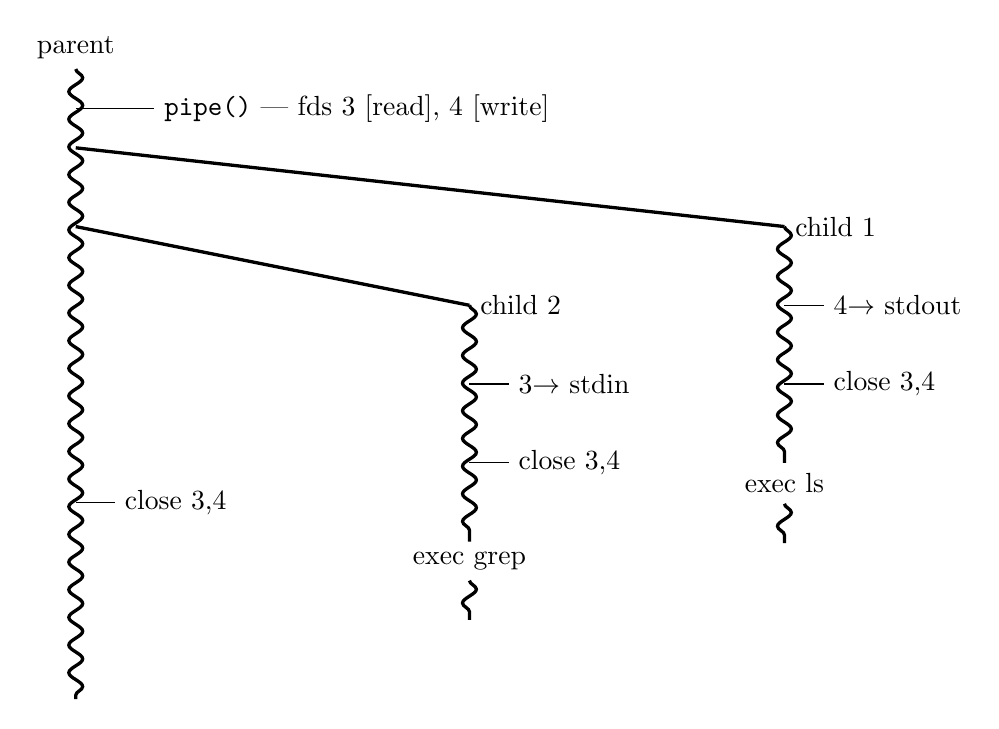
\begin{tikzpicture}
\tikzset{
    thread/.style={very thick,draw,decorate,decoration=snake},
    split/.style={very thick,draw},
    marker/.style={thin,draw},
}
\path[thread] (0, 0) --  (0, -8);
    \node[anchor=south] at (0,0) {parent};
\path[marker] (0, -.5) -- ++(1, 0) node[right] {\texttt{pipe()} --- fds 3 [read], 4 [write]};
    \path[split] (0, -1) --  (9, -2) node[right] {child 1};
    \path[marker] (9, -3) -- ++(.5, 0) node[right] {4$\rightarrow$ stdout};
    \path[marker] (9, -4) -- ++(.5, 0) node[right] {close 3,4};
    \path[thread] (9, -2) -- (9, -5) node[below] (exec ls) {exec ls};
    \path[thread] (exec ls.south) -- ++(0, -.5cm);

    \path[split] (0, -2) --  (5, -3) node[right] {child 2};
    \path[marker] (5, -4) -- ++(.5, 0) node[right] {3$\rightarrow$ stdin};
    \path[marker] (5, -5) -- ++(.5, 0) node[right] {close 3,4};
    \path[thread] (5, -3) -- (5, -6) node[below] (exec grep) {exec grep};
    \path[thread] (exec grep.south) -- ++(0, -.5cm);
    \path[marker] (0, -5.5) -- ++(.5, 0) node[right] {close 3,4};
\end{tikzpicture}
\end{frame}


% FIXME: better understanding that this works without write()/read() specifically?
